\label{sec:EFN}
Energy Flow Networks (EFN) and Particle Flow Networks (PFN) are neural networks that also operate with basic jet constituent information as input rather than reconstructed jets and multi-jet composites~\cite{Komiske:2018cqr}. The EFN structure takes only the rapidity, ${y}$, and azimuthal angle, ${\phi}$, of jet constituents as input, while the PFN takes the rapidity, azimuthal angle, and transverse momentum, $p_{T}$, of jet constituents as input. Both the EFN and PFN are two-component networks, and their internal structures are shown in Figure \ref{fig:EFNArch}. The implementations of the EFN and PFN used for di-Higgs classification use 200 nodes for each hidden layer in network (a), 256 nodes for the latent space dimension, and 300 nodes for each hidden layer in network (b). 

\begin{figure}[ht!]
\centering
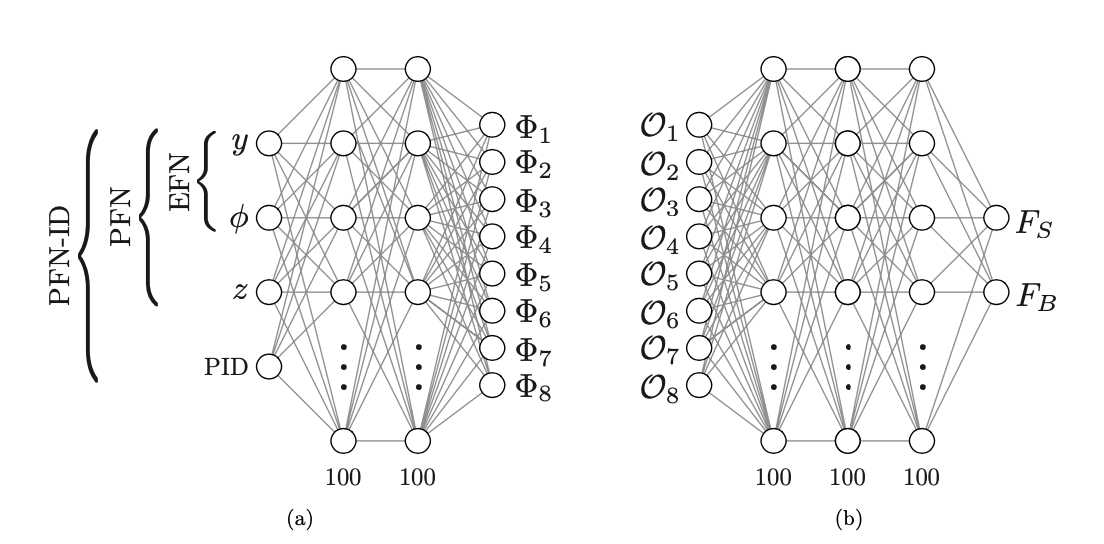
\includegraphics[scale=0.5]{./EFN/EFNArch.png}
\caption{Network (a) takes jet constituents information as input and outputs latent space $\Phi$ for each jet constituents. Network (b) takes $\mathcal{O}$, which is the linear combination of $\Phi$, as input and outputs final result.}
\label{fig:EFNArch}
\end{figure}

The EFN/PFN networks were trained using four separate categories split by number of jets and number of $b$-tags to test the network's dependence on higher-level jet information. Independent networks were trained using: all events, only events with $\geq$4 jets, only events with $\geq$4 jets and =2 $b$-tags, and only events with $\geq$4 jets and $\geq$4 $b$-tags. In each configuration, the number of signal and background events were adjusted to maintain an equal proportion of each population in the training sample. L2 regularization and dropout layers were added to minimize over-fitting. The results obtained from each EFN configuration are shown in Table~\ref{EFNtab}. The results of each PFN configuration are shown in Table~\ref{PFNtab}.

\begin{table}[ht!]
\centering
  %\begin{center}
    \begin{tabular}{|l|c|c|c|} % <-- Alignments: 1st column left, 2nd middle and 3rd right, with vertical lines in between
      \hline\hline
      \multirow{2}{*}{\textbf{Category}} & \multicolumn{3}{c|}{0PU}\\
      \cline{2-4}
      & Best $S/\sqrt{B}$ & \textbf{N$_{\mathrm{Signal}}$} & \textbf{N$_{\mathrm{Background}}$} \\
      \hline
      All Events & $1.407 \pm 0.006$ & $1.89\cdot 10^4$ & $1.80\cdot 10^8$ \\
      4Jets & $1.363 \pm 0.006$ & $1.63\cdot 10^4$ & $1.43\cdot 10^8$ \\
      4Jets 2BTags & $1.343 \pm 0.006$ & $1.33\cdot 10^4$ & $9.95\cdot 10^7$ \\
      4Jets 4BTags & $0.867 \pm 0.008$ & $3468.65$ & $1.60\cdot 10^7$ \\
      \hline\hline
    \end{tabular}
    \caption{EFN results. Normalized to full HL-LHC dataset of 3000 fb$^{-1}$}
  %\end{center}
\label{EFNtab}
\end{table}

\begin{table}[ht!]
\centering
  %\begin{center}
    \begin{tabular}{|l|c|c|c|} % <-- Alignments: 1st column left, 2nd middle and 3rd right, with vertical lines in between
      \hline\hline
      \multirow{2}{*}{\textbf{Category}} & \multicolumn{3}{c|}{0PU}\\
      \cline{2-4}
      & Best $S/\sqrt{B}$ & \textbf{N$_{\mathrm{Signal}}$} & \textbf{N$_{\mathrm{Background}}$} \\
      \hline
      All Events & $1.618 \pm 0.008$ & $1.79\cdot 10^4$ & $1.21\cdot 10^8$ \\
      4Jets & $1.580 \pm 0.008$ & $1.32\cdot 10^4$ & $7.00\cdot 10^7$ \\
      4Jets 2BTags & $1.574 \pm 0.009$ & $1.32\cdot 10^4$ & $4.85\cdot 10^7$ \\
      4Jets 4BTags & $0.903 \pm 0.009$ & $3297.34$ & $1.33\cdot 10^7$ \\
      \hline\hline
    \end{tabular}
    \caption{PFN results. Normalized to full HL-LHC dataset of 3000 fb$^{-1}$}
  %\end{center}
\label{PFNtab}
\end{table}

Both networks performed best when trained over all events without any cuts on the number of jets or $b$-tags. The EFN obtained a highest significance of 1.41$\pm$0.01, and the PFN obtained a highest significance of 1.62$\pm$0.01.
